\documentclass[sigconf,anonymous]{acmart}

\setcopyright{none}
\acmConference[ASP-DAC '27]{32nd Asia and South Pacific Design Automation Conference}{January 25--28, 2027}{Tokyo, Japan}
\acmYear{2027}
\copyrightyear{2027}
\acmDOI{}
\acmISBN{}

\usepackage{booktabs}
\usepackage{multirow}
\usepackage{array}
\usepackage{xspace}
\usepackage{enumitem}
\usepackage{tikz}
\usetikzlibrary{arrows.meta,positioning,fit}

\newcommand{\arch}{ArchXBench\xspace}
\newcommand{\cOne}{C1\xspace}
\newcommand{\cTwoG}{C2g\xspace}
\newcommand{\cFourI}{C4i\xspace}
\newcommand{\cFourTL}{C4tl\xspace}
\newcommand{\yes}{\textbf{3/3}}
\newcommand{\no}{0/3}
\definecolor{hmsolve}{RGB}{217,234,211}
\definecolor{hmpartial}{RGB}{255,242,204}
\definecolor{hmfail}{RGB}{244,204,204}
\definecolor{hmneutral}{RGB}{217,225,242}
\definecolor{codebg}{RGB}{235,248,250}
\definecolor{c1bar}{RGB}{91,155,213}
\definecolor{c2bar}{RGB}{237,125,49}
\definecolor{c4ibar}{RGB}{112,173,71}
\definecolor{c4tlbar}{RGB}{112,48,160}
\newcommand{\hmcell}[2]{\begingroup\setlength{\fboxsep}{1pt}\colorbox{#1}{\makebox[0.78cm][c]{\strut #2}}\endgroup}
\newcommand{\hmyes}{\hmcell{hmsolve}{\textbf{3/3}}}
\newcommand{\hmno}{\hmcell{hmfail}{0/3}}
\newcommand{\hmpart}[1]{\hmcell{hmpartial}{#1}}
\newcounter{rtlListing}
\emergencystretch=2em

\begin{document}

\title{Autonomous Synthesis of Hard RTL Designs via Iterative Repair and Modular Decomposition}

\author{Anonymous Author 1}
\affiliation{%
  \institution{Anonymous Institution}
  \country{Omitted for review}
}

\author{Anonymous Author 2}
\affiliation{%
  \institution{Anonymous Institution}
  \country{Omitted for review}
}

\author{Anonymous Author 3}
\affiliation{%
  \institution{Anonymous Institution}
  \country{Omitted for review}
}

\begin{abstract}
Large language models can generate short register-transfer level (RTL) fragments, but benchmark-level hardware synthesis requires executable correctness: simulation success, protocol consistency, and golden-output agreement.
\arch exposes this gap through a reported hard-task frontier beginning at Level~4 under direct prompting.
This paper evaluates whether verifier-grounded autonomous synthesis can cross that frontier without confusing model failures with benchmark-contract failures.
Four conditions are compared on \arch Levels~3--6: single-shot generation (\cOne), monolithic golden-feedback repair (\cTwoG), decomposition-guided iterative repair (\cFourI), and testbench-localized decomposition (\cFourTL).
\cFourI solves five Level-3 numerical kernels at 3/3 seeds where both \cOne and \cTwoG fail.
\cFourTL solves all four core Level-4 designs, including 16-point FFT/IFFT, at 5/5 seeds.
Golden-verified Level-5 and Level-6 solves are obtained on convolution, image-processing, and AES designs.
Decomposition is not universally superior: \cTwoG solves several Level-5 rows that decomposed methods do not.
The central contribution is an executable-contract-aware synthesis methodology: original-benchmark solves, minimally repaired executable contracts, and held rows are separated before success is claimed.
Code, prompts, logs, generated RTL, and result JSONs are prepared for anonymous artifact release.\footnote{Repository URL withheld for double-blind review.}
\end{abstract}

\begin{CCSXML}
<ccs2012>
<concept>
<concept_id>10010520.10010553.10010562</concept_id>
<concept_desc>Computer systems organization~Embedded systems</concept_desc>
<concept_significance>500</concept_significance>
</concept>
<concept>
<concept_id>10010520.10010575.10010755</concept_id>
<concept_desc>Computer systems organization~Reliability</concept_desc>
<concept_significance>300</concept_significance>
</concept>
</ccs2012>
\end{CCSXML}

\ccsdesc[500]{Hardware~Hardware description languages and compilation}
\ccsdesc[500]{Hardware~Electronic design automation}
\ccsdesc[300]{Software and its engineering~Automatic programming}

\keywords{benchmark evaluation, CEGIS, hardware verification, LLM agents, RTL synthesis, Verilog generation}

\maketitle

\section{Introduction}

\begin{figure}[t]
\centering
\resizebox{\columnwidth}{!}{%
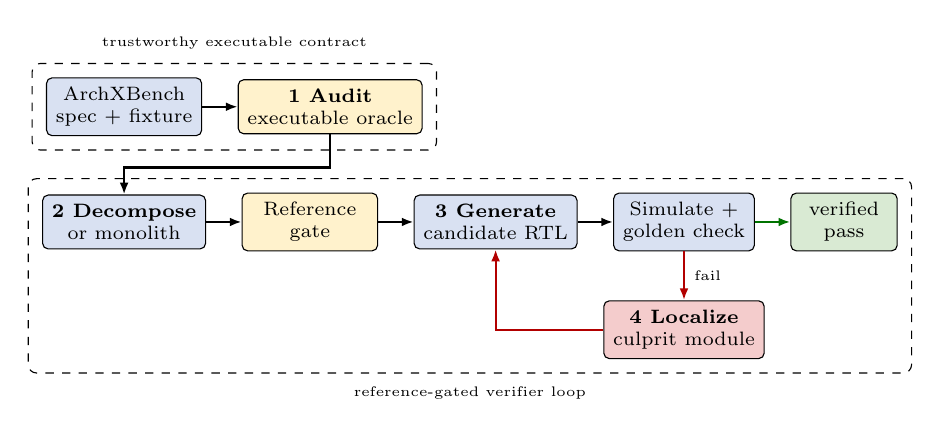
\begin{tikzpicture}[
    node distance=0.42cm and 0.45cm,
    stage/.style={draw, rounded corners=2pt, align=center, minimum width=1.72cm, minimum height=0.60cm, font=\scriptsize, fill=hmneutral},
    gatebox/.style={draw, rounded corners=2pt, align=center, minimum width=1.72cm, minimum height=0.60cm, font=\scriptsize, fill=hmpartial},
    passbox/.style={draw, rounded corners=2pt, align=center, minimum width=1.35cm, minimum height=0.54cm, font=\scriptsize, fill=hmsolve},
    failbox/.style={draw, rounded corners=2pt, align=center, minimum width=1.72cm, minimum height=0.60cm, font=\scriptsize, fill=hmfail},
    lane/.style={draw, rounded corners=3pt, dashed, inner sep=5pt},
    arrow/.style={-{Latex[length=1.5mm]}, thick},
    failarrow/.style={-{Latex[length=1.5mm]}, thick, draw=red!70!black},
    passarrow/.style={-{Latex[length=1.5mm]}, thick, draw=green!45!black}
]
\node[stage] (spec) {ArchXBench\\spec + fixture};
\node[gatebox, right=of spec] (audit) {\textbf{1 Audit}\\executable oracle};
\node[stage, below=0.74cm of spec] (decomp) {\textbf{2 Decompose}\\or monolith};
\node[gatebox, right=of decomp] (gate) {Reference\\gate};
\node[stage, right=of gate] (impl) {\textbf{3 Generate}\\candidate RTL};
\node[stage, right=of impl] (sim) {Simulate +\\golden check};
\node[passbox, right=of sim] (pass) {verified\\pass};
\node[failbox, below=0.62cm of sim] (feedback) {\textbf{4 Localize}\\culprit module};
\draw[arrow] (spec) -- (audit);
\path (audit.south) -- ++(0,-0.42cm) coordinate (auditdown);
\draw[arrow] (audit.south) -- (auditdown) -| (decomp.north);
\draw[arrow] (decomp) -- (gate);
\draw[arrow] (gate) -- (impl);
\draw[arrow] (impl) -- (sim);
\draw[passarrow] (sim) -- (pass);
\draw[failarrow] (sim) -- node[right,font=\tiny] {fail} (feedback);
\path (feedback.west) -- ++(-0.38cm,0) coordinate (fbleft);
\path (impl.south) -- ++(0,-0.72cm) coordinate (impldown);
\draw[failarrow] (feedback.west) -- (fbleft) -| (impldown) -- (impl.south);
\node[lane, fit=(spec)(audit)] (trust) {};
\node[lane, fit=(decomp)(gate)(impl)(sim)(feedback)(pass)(fbleft)(impldown)] (synth) {};
\node[font=\tiny, above=0.5mm of trust] {trustworthy executable contract};
\node[font=\tiny, below=0.5mm of synth] {reference-gated verifier loop};
\end{tikzpicture}
}
\Description{Pipeline with two lanes: trustworthy contract audit followed by verifier-grounded decomposition, reference validation, RTL generation, golden checking, fault localization, and targeted repair.}
\caption{\cFourTL pipeline: audit the executable contract, validate references, then repair only the localized culprit module.}
\label{fig:pipeline}
\end{figure}

Autonomous code agents close executable loops: generate a candidate, run a checker, inspect failures, and repair.
For software tasks, this loop has changed what counts as a meaningful benchmark result.
For hardware design, the question is harder: can an autonomous agent synthesize RTL that survives simulation, protocol assumptions, and golden-output comparison?

RTL correctness depends on bit widths, signedness, clocking, reset protocols, pipeline latency, and streaming handshakes.
Hard RTL synthesis therefore tests whether autonomous agents can handle low-level, state-dependent, timing-sensitive design, not just surface-level code generation.
The severity is practical: an RTL generator that compiles but mishandles latency, signed arithmetic, or output encoding can pass superficial checks while producing unusable hardware.

This paper studies the problem on \arch, a benchmark suite for complex RTL synthesis~\cite{purini2025archxbench}.
Unlike VerilogEval~\cite{liu2023verilogeval} and RTLLM~\cite{lu2023rtllm}, which target smaller designs, \arch spans arithmetic kernels, FFTs, filters, image processing, matrix multiplication, and cryptography across six difficulty levels.
The \arch paper reports a direct-generation frontier beginning at Level~4: lower levels are broadly reachable, while hard Level-4 rows such as FFT/IFFT expose near-zero zero-shot pass@5 behavior.
If an autonomous synthesis loop can solve rows beyond it, the evaluation question changes from ``can an LLM emit a complete design in one shot?'' to ``can a verifier-grounded agent converge to correct RTL?''

The central question is: \emph{can verifier-grounded autonomous synthesis solve hard RTL benchmark tasks that direct generation does not solve, while maintaining a clear distinction between model failures and benchmark-contract failures?}
The answer is yes, but not through a single universally dominant architecture.
\cFourI solves five Level-3 numerical kernels at 3/3 seeds where \cOne and \cTwoG both fail.
\cFourTL solves all four core Level-4 designs at 5/5 seeds, including the 16-point FFT and IFFT.
Golden-verified solves extend to Level-5 convolution and image processing and to Level-6 AES encryption and decryption.
At the same time, \cTwoG is a strong baseline: it solves several Level-5 rows and multiple repaired-contract designs that decomposed methods do not.
The contribution is not a claim that decomposition dominates monolithic repair.
It is evidence that verifier-grounded synthesis, in both monolithic and decomposed forms, can cross parts of the reported hard-task frontier, and that benchmark contracts must be audited before either successes or failures are interpreted.

This paper makes three contributions:
\begin{enumerate}[leftmargin=*]
    \item The proposed work introduces an executable-contract-aware evaluation discipline for autonomous RTL synthesis: released contracts, minimally repaired executable contracts, and held rows are separated before positive claims are made.
    \item The proposed work gives a verifier-grounded synthesis algorithm that instantiates direct generation, monolithic repair, decomposition-guided repair, and testbench-localized repair as controlled ablations of feedback, decomposition, reference validation, and localization.
    \item The proposed work demonstrates hard \arch solves beyond the reported direct-generation frontier, including robust Level-4 original-contract FFT/IFFT solves and golden-verified Level-5/Level-6 solves.
\end{enumerate}

\section{Related Work}

\subsection{LLM-Based RTL Generation}

VerilogEval and RTLLM made Verilog generation measurable with automatic checking~\cite{liu2023verilogeval,lu2023rtllm}.
Subsequent systems add feedback, planning, workflow search, or evolutionary search for RTL generation and repair~\cite{thakur2024autochip,ho2024verilogcoder,tan2025autoverifix,spec2rtlagent2025,wei2025vflow,min2025revolution}.
Recent benchmark and verification work further shows that flawed executable contracts and weak oracles can distort RTL evaluation~\cite{wang2026rtlbenchmt,li2026formalrtl,wang2026rtlbenchls}.
Table~\ref{tab:positioning} summarizes where the present study sits.

\begin{table*}[t]
\centering
\caption{Positioning relative to recent LLM-aided RTL work. The key distinction is a hard-\arch study that combines verifier-grounded synthesis with explicit original-contract versus repaired-contract accounting.}
\label{tab:positioning}
\footnotesize
\setlength{\tabcolsep}{3.4pt}
\renewcommand{\arraystretch}{1.08}
\begin{tabular}{p{2.6cm}p{3.4cm}p{3.0cm}p{5.0cm}}
\toprule
Line of work & Examples & Main strength & Gap addressed here \\
\midrule
RTL benchmarks & VerilogEval, RTLLM & Automatic functional checks & Harder \arch L3--L6 rows \\
Agentic RTL generation & AutoChip, VerilogCoder, AutoVeriFix, Spec2RTL & Feedback, planning, tracing & Original vs repaired contract accounting \\
Workflow/search & VFlow, REvolution & Workflow and population search & Hard-frontier executable synthesis study \\
Benchmark/oracle validity & RTL-BenchMT, FormalRTL, RTL-BenchLS & Maintenance, formal oracles & Contract audit tied to synthesis claims \\
This work & \cOne/\cTwoG/\cFourI/\cFourTL on \arch & Golden repair, decomposition, localization & Cross frontier while separating held rows \\
\bottomrule
\end{tabular}
\renewcommand{\arraystretch}{1.0}
\end{table*}

Our work evaluates on \arch Levels~3--6, including rows at and above the reported Level-4 frontier.
It separates original benchmark contracts from repaired executable contracts so that model failures are not confused with stale testbenches, file-format mismatches, or inconsistent golden comparators.

\subsection{Verifier-Grounded Synthesis}

Counterexample-guided inductive synthesis (CEGIS) uses a verifier to reject incorrect candidates and guide the next attempt.
LLM-based repair loops instantiate a related pattern: generate code, run tests, inspect errors, and repair.
For RTL, verifier feedback is heterogeneous: failures arise from syntax, elaboration, simulation, timing, protocol mismatch, file-output mismatch, or incorrect golden references.
The present pipeline treats simulator and golden-output feedback as first-class signals and audits the benchmark contract when executable artifacts disagree.

\section{Problem Setting}

Each \arch design provides a natural-language specification and executable assets: Verilog testbenches, input files, output files, and comparison scripts.
An autonomous synthesis condition receives the task and emits RTL.
For self-checking designs, a run succeeds only when the official testbench passes all checks.
For file-output designs, simulation completion is not sufficient; the generated output must match the golden output element by element.

Three evaluation classes are distinguished:
\begin{itemize}[leftmargin=*]
    \item \textbf{Original-contract results:} runs against the released benchmark as-is.
    \item \textbf{Repaired-contract results:} runs against a copied fixture with minimally repaired infrastructure inconsistencies.
    \item \textbf{Held or excluded rows:} tasks where the released contract remains too ambiguous for a credible positive result.
\end{itemize}

\begin{figure}[!ht]
\centering
\scriptsize
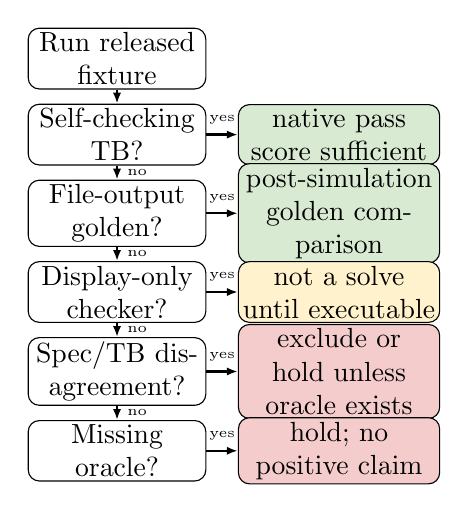
\begin{tikzpicture}[
node distance=1.8mm,
q/.style={draw,rounded corners,align=center,text width=2.15cm,minimum height=5.5mm,inner sep=1.5pt},
a/.style={draw,rounded corners,fill=hmsolve,align=center,text width=2.45cm,minimum height=5.5mm,inner sep=1.5pt},
h/.style={draw,rounded corners,fill=hmpartial,align=center,text width=2.45cm,minimum height=5.5mm,inner sep=1.5pt},
bad/.style={draw,rounded corners,fill=hmfail,align=center,text width=2.45cm,minimum height=5.5mm,inner sep=1.5pt},
arr/.style={-{Latex[length=1.4mm]},thick}
]
\node[q] (run) {Run released fixture};
\node[q, below=of run] (self) {Self-checking TB?};
\node[a, right=4mm of self] (native) {native pass score sufficient};
\node[q, below=of self] (file) {File-output golden?};
\node[a, right=4mm of file] (golden) {post-simulation golden comparison};
\node[q, below=of file] (display) {Display-only checker?};
\node[h, right=4mm of display] (nosolve) {not a solve until executable};
\node[q, below=of display] (spec) {Spec/TB disagreement?};
\node[bad, right=4mm of spec] (exclude) {exclude or hold unless oracle exists};
\node[q, below=of spec] (oracle) {Missing oracle?};
\node[bad, right=4mm of oracle] (hold) {hold; no positive claim};
\draw[arr] (run) -- (self);
\draw[arr] (self) -- node[above,font=\tiny] {yes} (native);
\draw[arr] (self) -- node[right,font=\tiny] {no} (file);
\draw[arr] (file) -- node[above,font=\tiny] {yes} (golden);
\draw[arr] (file) -- node[right,font=\tiny] {no} (display);
\draw[arr] (display) -- node[above,font=\tiny] {yes} (nosolve);
\draw[arr] (display) -- node[right,font=\tiny] {no} (spec);
\draw[arr] (spec) -- node[above,font=\tiny] {yes} (exclude);
\draw[arr] (spec) -- node[right,font=\tiny] {no} (oracle);
\draw[arr] (oracle) -- node[above,font=\tiny] {yes} (hold);
\end{tikzpicture}
\caption{Executable-contract classification. Positive results are claimed only when the released or repaired fixture has an executable oracle.}
\Description{Flowchart classifying benchmark fixtures as self-checking, file-output with golden comparison, display-only, specification-disagreeing, or missing-oracle cases.}
\label{fig:contracts}
\end{figure}

\section{Method}

\subsection{Evaluated Conditions}

The condition grid below summarizes the operational differences among the four conditions.
All conditions receive the same specification, module interface, and released testbench.
The difference is how much executable feedback enters the loop and whether the design is treated as a monolith or decomposed into modules.
Thus the four conditions are also ablations: \cOne removes feedback, \cTwoG removes decomposition, \cFourI adds decomposition without localized repair, and \cFourTL adds a strict reference gate plus localization.

\begin{center}
\centering
\footnotesize\textbf{Condition grid.} Operational differences among synthesis conditions. ``Ref.\ gate'' indicates whether the decomposition's reference composition must pass the system testbench before synthesis proceeds. ``Local repair'' describes repair granularity.
\par
\scriptsize
\setlength{\tabcolsep}{3.0pt}
\begin{tabular}{lccccc}
\toprule
Cond. & Decomp. & Ref.\ gate & Golden fb. & Local repair & Budget \\
\midrule
\cOne & no & -- & no & -- & 5 shots \\
\cTwoG & no & -- & yes & whole design & 30 rounds \\
\cFourI & yes & sanity & yes & per module & $\approx$28 rds \\
\cFourTL & yes & strict & yes & culprit only & 3+$\approx$28 rds \\
\bottomrule
\end{tabular}
\end{center}

\begin{table*}[t]
\centering
\caption{Executable-contract-aware verifier-grounded RTL synthesis. The condition parameter selects \cOne, \cTwoG, \cFourI, or \cFourTL by enabling feedback, decomposition, reference gating, and localization.}
\label{alg:synthesis}
\footnotesize
\setlength{\tabcolsep}{5pt}
\renewcommand{\arraystretch}{1.12}
\begin{tabular}{p{1.35cm}p{13.6cm}}
\toprule
\textbf{Input} & Specification $S$, released fixture $B$, condition $c$, seed $s$, budget $T$ \\
\textbf{Output} & \textsc{solved}, \textsc{unsolved}, or \textsc{held}, with saved artifact record \\
\midrule
\textbf{Audit} & Classify $B$ using Fig.~\ref{fig:contracts}. If no executable oracle can be recovered, return \textsc{held}. \\
\textbf{Decompose} & If $c$ uses decomposition, request interfaces, top wrapper, and reference modules $R_1,\ldots,R_n$; otherwise set $n=1$ and target the whole design. \\
\textbf{Gate} & When enabled, simulate the composed references against $B$; retry with failure feedback and abort if no valid reference composition is found. \\
\textbf{Generate} & Produce candidate RTL modules $M_1,\ldots,M_n$ from $S$, $B$, references, and seed $s$. \\
\textbf{Verify} & For each round $t \leq T$, simulate the composed candidate and compute pass/golden score. If all checks pass, save RTL and return \textsc{solved}. \\
\textbf{Localize} & Select a repair target: \cTwoG selects the whole design; \cFourI selects the next module in fixed order; \cFourTL swaps each $M_i$ with $R_i$ and selects the module with the largest system-score improvement. \\
\textbf{Repair} & Repair only the selected target using compile errors, failing indices, expected/actual values, swap scores, and the relevant reference; then repeat verification. \\
\textbf{Exit} & Save the final artifact and return \textsc{unsolved}. \\
\bottomrule
\end{tabular}
\renewcommand{\arraystretch}{1.0}
\end{table*}

\textbf{\cOne: direct generation.}
The model receives the specification and testbench excerpt and emits five independent RTL candidates.
The highest-scoring candidate is retained; no repair feedback is used.

\textbf{\cTwoG: monolithic golden-feedback repair.}
The model emits a complete top module, then iteratively repairs it using compile errors, self-check failures, and golden-output mismatches with expected-versus-actual indices.
The loop terminates when all checks pass or after 30 rounds; long conversations are pruned to the first two and last sixteen messages.
This is a deliberately strong baseline because it uses the same executable oracle as decomposed methods without paying module-integration risk.

\textbf{\cFourI: decomposition-guided iterative repair.}
\cFourI decomposes the task into 3--7 submodules with explicit interfaces, a top-level wrapper, and reference implementations.
After a reference-composition sanity check, submodules are solved in fixed order.
During submodule repair, unsolved neighbors are held at their references, isolating bugs to the target module; each of $n$ submodules receives $\lfloor 28/n \rfloor$ repair rounds.

\textbf{\cFourTL: testbench-localized decomposed repair.}
\cFourTL uses the same decomposition structure as \cFourI but adds two mechanisms: a strict reference gate and trace-lifted fault localization.

The reference gate requires the composed reference implementation to pass the system-level testbench before synthesis begins; failed references are retried up to three times, otherwise the run aborts.
After candidate generation, \cFourTL localizes a failure by swapping each candidate submodule with its validated reference while all other candidates remain fixed.
Let $M$ denote the current composed candidate and $M^{(i\leftarrow R_i)}$ denote replacing only module $i$ with its validated reference.
For executable score function $q(\cdot)$, \cFourTL computes
\begingroup
\setlength{\abovedisplayskip}{3pt}
\setlength{\belowdisplayskip}{3pt}
\setlength{\abovedisplayshortskip}{3pt}
\setlength{\belowdisplayshortskip}{3pt}
\[
\Delta_i = q(M^{(i\leftarrow R_i)}) - q(M), \qquad
i^\star = \arg\max_i \Delta_i .
\]
\endgroup
The selected module $M_{i^\star}$ is repaired using simulator output, golden mismatches, swap scores, and the reference implementation.
The prompt asks the model to trace the first failing datapath, compute expected intermediate values, identify the root cause, and then fix.

The localization mechanism is the central algorithmic distinction.
\cFourI repairs modules in a fixed order; \cFourTL uses system-level evidence to identify which module is most implicated.
For tightly coupled pipelines such as the 16-point FFT, this targeted approach avoids diffuse repair of modules that may not be at fault.
The localization step is heuristic rather than a correctness guarantee.
It is strongest when the reference composition is valid and one module dominates the observed failure.
It can be misled by coupled multi-module bugs, bad decompositions, or errors whose effects are masked until multiple modules are replaced together.

\subsection{Artifact and Verification Discipline}

Each run is recorded under a repository artifact tree with a structured result file containing the design, condition, model, seed, pass counts, golden counts, LLM-call count, wall time, and generated RTL.
File-output designs require strict golden verification: the generated output is compared element by element against the golden reference with a tolerance of $\pm 1$ on integer values.
Native simulation completion alone is treated as diagnostic evidence, not as a solve.

\section{Experimental Setup}

\subsection{Benchmark Scope}

The evaluation covers \arch Levels~3--6: iterative arithmetic, FFT/IFFT, floating-point pipelines, FIR filters, image-processing kernels, matrix multiplication, and AES.
Lower levels are excluded because the \arch paper reports that current models already solve them.
Execution uses repository scripts with Python orchestration, Icarus Verilog (\texttt{iverilog}), and the VVP runtime (\texttt{vvp}); each candidate is compiled before simulation and self-checking or golden-output comparison.

\subsection{Seeds, Model, and Metrics}

Main tables use seeds 42, 123, and 456.
Two additional seeds (789, 1024) provide robustness evidence for \cFourTL Level-4 rows.
These are fixed seeds chosen for reproducibility, not tuned seeds.
\cOne uses five seeds for the two borderline Level-3 floating-point rows, \texttt{fp\_adder} and \texttt{fp\_multiplier}, to give a stricter direct-generation baseline estimate.
The primary model is GPT-5.5 as recorded in the repository artifacts.

For run $r$, let $p_r/t_r$ denote native self-checking passes and $g_r/h_r$ denote golden-output matches.
The executable score is
\[
q(r)=
\begin{cases}
g_r/h_r, & h_r>0,\\
p_r/t_r, & h_r=0 \text{ and } t_r>0,\\
0, & \text{otherwise}.
\end{cases}
\]
Run $r$ solves iff $q(r)=1$.
For design $d$, condition $c$, and seed set $S$, full-row and partial-row indicators are
\[
F_{d,c}=\prod_{s\in S}\mathbf{1}[q(d,c,s)=1],
\qquad
P_{d,c}=\mathbf{1}\!\left[\max_{s\in S} q(d,c,s)=1\right]-F_{d,c}.
\]
Figure~\ref{fig:solve-rate} reports these design-row rates by level.

All methods run as executable synthesis loops; the method budgets are summarized in the condition grid in Section~4.1.
The Level-4 FFT solves in roughly 5 minutes and 6 LLM calls, while harder designs such as \texttt{harris\_corner\_detection} require 10.7 calls and 9.4 minutes on average.
Failed decomposed runs typically consume the full repair budget: failed \cFourI/\cFourTL-style rows in the FFT/IFFT diagnostics use about 26--29 LLM calls and can take roughly 20--45 minutes on the local runner.

\section{Crossing the Original-Contract Frontier}

Table~\ref{tab:original-main} reports the main original-contract results.

\begin{figure}[t]
\centering
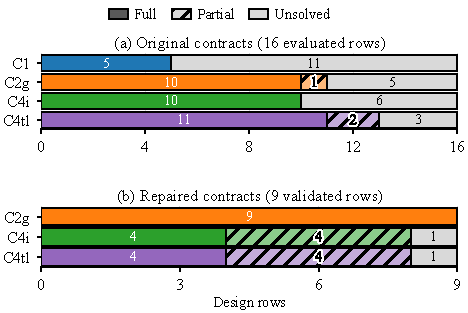
\includegraphics[width=\columnwidth]{figures/fig3_solve_rate.pdf}
\Description{Stacked grouped bar chart showing original-contract row solve rates by ArchXBench level for C1, C2g, C4i, and C4tl. Colors encode synthesis condition. Solid bars show rows solved on all main seeds; hatched extensions show rows where at least one seed solves but not all main seeds solve.}
\caption{Original-contract solve rate by level. Colors encode synthesis condition. Solid bars count rows solved on all main seeds; hatched segments count partial rows where at least one seed passes but not all main seeds pass.}
\label{fig:solve-rate}
\end{figure}

\textbf{Level 3.}
\cFourI provides the strongest method-value evidence: it solves five numerical kernels at 3/3 seeds where \cOne scores 0/3--0/5 and \cTwoG scores 0/3--1/5.
\cFourTL matches \cFourI on four of five rows but solves \texttt{gauss\_siedel} at only 1/3.
For context, \cFourI decomposes \texttt{gauss\_siedel} into three submodules (reciprocal unit, iteration step, solution selector), allowing each to be solved and tested in isolation.
The negative result on \texttt{newton\_raphson\_polynomial} is an original-checker ceiling: three of its 100 assertions are structurally unsatisfiable, capping the achievable score at 97/100.
After removing only those three unsatisfiable residual assertions in the repaired-contract fixture, \cTwoG solves all three seeds (Table~\ref{tab:repaired}), confirming that the design itself is within model capability.

\textbf{Level 4.}
\cFourTL solves all four core Level-4 rows at 3/3 main seeds and 2/2 robustness seeds, for 5/5 total.
The 16-point FFT and IFFT rows are the strongest hard-frontier evidence because they are self-checking original-contract solves with no benchmark repair.
\cFourTL decomposes \texttt{fft\_16pt\_iterative} into four submodules (bit-reverse mapper, twiddle ROM, butterfly unit, output scaler) and uses trace-lifted localization to identify which module is at fault after each simulation failure.
\cTwoG also solves the FFT/IFFT rows at 3/3; \cFourI does not.
\cTwoG avoids the module-order problem by repairing the design monolithically; \cFourTL retains modular structure but uses swap-based localization to avoid spending repair budget on modules that already compose correctly.
\cFourI's fixed sequential repair order can spend iterations on modules that already compose correctly while the actual fault remains in a later module; \cFourTL's swap-based localization directly identifies the culprit before repair.
The pipeline rows (\texttt{fp\_adder\_pipeline}, \texttt{fp\_mult\_pipeline}) are solved by all conditions.

\textbf{Levels 5--6.}
\cFourI obtains 3/3 golden-verified solves on \texttt{conv1d}, \texttt{harris\_corner\_detection}, and both AES rows.
\cFourI decomposes AES encryption into six submodules (S-box, SubBytes, ShiftRows, MixColumns, round function, key expansion), each implemented and tested against the system testbench with other modules held at their references.
Several Level-5 rows are solved only by \cTwoG: \texttt{conv2d} (4{,}096/4{,}096), \texttt{dct\_idct\_8pt\_pipelined} (16/16), and \texttt{unsharp\_mask} (65{,}536/65{,}536).
These rows demonstrate that monolithic repair is the stronger strategy when the design is compact enough for whole-design feedback or when the primary difficulty is a global convention such as file format or fixed-point encoding.

\begin{table*}[t]
\centering
\caption{Original-contract result heatmap on \arch. Green cells solve all main seeds; yellow cells are partial; red cells fail. GV marks golden-verified file-output rows. Level-4 \cFourTL rows additionally solve robustness seeds 789 and 1024, giving 5/5 total.}
\label{tab:original-main}
\scriptsize
\setlength{\tabcolsep}{3.0pt}
\begin{tabular}{llccccp{2.7cm}}
\toprule
Level & Design & \cOne & \cTwoG & \cFourI & \cFourTL & Evidence \\
\midrule
L3 & \texttt{fp\_adder} & \hmcell{hmfail}{0/5} & \hmpart{1/5} & \hmyes & \hmyes & decomposition wins \\
L3 & \texttt{fp\_multiplier} & \hmcell{hmfail}{0/5} & \hmno & \hmyes & \hmyes & decomposition wins \\
L3 & \texttt{gauss\_siedel} & \hmno & \hmno & \hmyes & \hmpart{1/3} & \cFourI strongest \\
L3 & \texttt{gradient\_descent} & \hmno & \hmno & \hmyes & \hmyes & decomposition wins \\
L3 & \texttt{newton\_raphson\_sqrt} & \hmno & \hmno & \hmyes & \hmyes & decomposition wins \\
L3 & \texttt{newton\_raphson\_polynomial} & \hmno & \hmno & \hmno & \hmno & checker ceiling at 97/100 \\
\midrule
L4 & \texttt{fft\_16pt\_iterative} & \hmno & \hmyes & \hmno & \hmyes & hard-row solve; 5/5 \\
L4 & \texttt{ifft\_16pt\_iterative} & \hmno & \hmyes & \hmno & \hmyes & hard-row solve; 5/5 \\
L4 & \texttt{fp\_adder\_pipeline} & \hmyes & \hmyes & \hmyes & \hmyes & all methods solve; 5/5 \\
L4 & \texttt{fp\_mult\_pipeline} & \hmyes & \hmyes & \hmyes & \hmyes & all methods solve; 5/5 \\
\midrule
L5 & \texttt{conv1d} & \hmyes & \hmyes & \hmyes & \hmpart{1/3} & GV \\
L5 & \texttt{conv2d} & \hmno & \hmyes & \hmno & \hmno & GV; \cTwoG strongest \\
L5 & \texttt{dct\_idct\_8pt\_pipelined} & \hmno & \hmyes & \hmno & \hmno & GV; \cTwoG strongest \\
L5 & \texttt{harris\_corner\_detection} & \hmno & \hmyes & \hmyes & \hmno & GV \\
L5 & \texttt{unsharp\_mask} & \hmno & \hmyes & \hmno & \hmno & GV; \cTwoG strongest \\
\midrule
L6 & \texttt{aes\_encryption} & \hmyes & \hmyes & \hmyes & \hmpart{2/3} & GV \\
L6 & \texttt{aes\_decryption} & \hmpart{1/3} & \hmyes & \hmyes & \hmpart{1/3} & GV; repair improves C1 \\
\bottomrule
\end{tabular}
\end{table*}

The results are not presented as a universal decomposition win.
\cTwoG is a serious baseline: it matches or outperforms decomposition on 8 of 17 original-contract rows.
The most accurate interpretation is that decomposition provides value on specific hard rows and gives a structured synthesis process, while monolithic golden-feedback repair is often sufficient and sometimes better.

\begin{table}[t]
\centering
\caption{Second-model validation with Claude Sonnet 5 on selected hard-frontier rows. GV denotes golden-verified file-output rows.}
\label{tab:sonnet}
\scriptsize
\setlength{\tabcolsep}{4pt}
\begin{tabular}{lcc}
\toprule
Design & \cTwoG & \cFourTL \\
\midrule
\texttt{fft\_16pt\_iterative} & \yes & \yes \\
\texttt{ifft\_16pt\_iterative} & \yes & \yes \\
\texttt{aes\_encryption} & \yes\ GV & \no\ GV \\
\texttt{aes\_decryption} & \yes\ GV & \no\ GV \\
\bottomrule
\end{tabular}
\end{table}

\textbf{Model generality.}
To test whether the hard-frontier result is specific to \texttt{gpt-5.5}, Table~\ref{tab:sonnet} repeats the strongest original-contract rows with Claude Sonnet 5.
The original Level-4 FFT/IFFT rows solve on all three seeds under both \cTwoG and \cFourTL, and the Level-6 AES rows solve on all three seeds under \cTwoG with golden verification.
Sonnet 5 does not solve AES under \cFourTL because the reference decomposition fails before localized repair can begin.
For AES encryption, Sonnet 5 produces decompositions whose reference compositions fail the original system testbench; for AES decryption, it does not produce a usable reference composition within the generation budget.
This indicates model-dependent sensitivity in the decomposition gate, while monolithic golden-feedback repair remains robust on the same AES rows.

\textbf{Case study: original Level-4 FFT.}
\texttt{fft\_16pt\_iterative} is a self-checking original-contract row, so no benchmark repair is involved.
\cOne fails on all three main seeds, while \cTwoG and \cFourTL solve all three.
The row therefore isolates the central mechanism: executable feedback can turn a direct-generation failure into a verified RTL solve without changing the released checker.
In one robustness seed, \cFourTL localizes a 9/33 failure to the butterfly while the twiddle ROM, index generator, and bit-reversal modules each pass in isolation; one repair then passes all 33 checks.
The repaired RTL explicitly implements signed Q1.15 complex rotation.

\par\addvspace{0.35\baselineskip}
\begin{center}
\refstepcounter{rtlListing}
\footnotesize\textbf{Listing~\thertlListing.} Generated RTL excerpt from the Level-4 FFT butterfly repair.\label{lst:rtl-snippet}

\fcolorbox{black!25}{codebg}{%
\begin{minipage}{0.94\columnwidth}
{\scriptsize\ttfamily
assign prod\_rr = b\_real * tw\_cos\_q15;\\
assign prod\_is = b\_imag * tw\_sin\_q15;\\
assign prod\_ic = b\_imag * tw\_cos\_q15;\\
assign prod\_rs = b\_real * tw\_sin\_q15;\\
assign rot\_real\_w = (prod\_rr - prod\_is + ROUND) \textgreater{}\textgreater{}\textgreater{} 15;\\
assign rot\_imag\_w = (prod\_ic + prod\_rs + ROUND) \textgreater{}\textgreater{}\textgreater{} 15;\\
assign y0\_real = a\_real + rot\_real;\quad assign y1\_real = a\_real - rot\_real;\\
assign y0\_imag = a\_imag + rot\_imag;\quad assign y1\_imag = a\_imag - rot\_imag;
}
\end{minipage}
}
\end{center}
\par\addvspace{0.35\baselineskip}

\section{Executable-Contract Audit}

Hard RTL benchmarks are useful only when their executable contracts reflect the intended task.
During evaluation, several rows were found to contain inconsistent specifications, stale comparators, display-only checkers, or output-schema mismatches.
The released benchmark is not overwritten.
Repaired fixtures are kept under a separate artifact root and reported separately.

The audit follows a fixed protocol.
First, the released fixture is run unchanged.
Second, the checker is classified (self-checking, file-output with golden, display-only, stale, specification-inconsistent, or missing-oracle).
Third, file-output rows are judged only by post-simulation golden comparison.
Fourth, infrastructure repairs are applied only in copied fixtures and only when the intended oracle is recoverable from released assets.
Fifth, unresolved rows are held rather than converted into positive results.
The repair rule is intentionally narrow: a repaired fixture may make an existing oracle executable or repair file-format infrastructure, but it may not change the semantic task, introduce hidden target behavior, or move a row into the original-contract table.

\par\addvspace{0.30\baselineskip}
\noindent\begin{minipage}{\columnwidth}
\refstepcounter{table}
\label{tab:repaired}
\footnotesize\textbf{Table~\thetable.} Repaired-contract results. These are separate from original \arch claims.
\par
\centering
\footnotesize
\setlength{\tabcolsep}{4.0pt}
\renewcommand{\arraystretch}{0.92}
\begin{tabular}{lccc}
\toprule
Design & \cTwoG & \cFourI & \cFourTL \\
\midrule
\texttt{conv\_3d} & 3/3 & 2/3 & 0/3 \\
\texttt{multich\_conv2d} & 3/3 & 3/3 & 3/3 \\
\texttt{quantized\_matmul} & 3/3 & 3/3 & 0/3 \\
\texttt{fp\_band\_pass\_fir} & 3/3 & 0/1 & 0/1 \\
\texttt{fp\_high\_pass\_fir} & 3/3 & 0/1 & 0/1 \\
\texttt{newton\_raphson\_polynomial} & 3/3 & 1/3 & 1/3 \\
\texttt{systolic\_gemm} & 0/3 & 0/3 & 0/3 \\
\bottomrule
\end{tabular}
\renewcommand{\arraystretch}{1.0}
\end{minipage}
\par\addvspace{0.55\baselineskip}

The audit produces both positive and negative evidence.
Repairing the executable contract for \texttt{multich\_conv2d} and \texttt{quantized\_matmul} makes the intended task measurable and solvable.
By contrast, converting the display-only \texttt{systolic\_gemm} checker into executable checks does not produce a win: all methods remain at \no.
This is a genuine remaining capability boundary, not a benchmark-repair success.

Several rows remain held or excluded.
The L4 FIR family is excluded because the specification and testbench disagree on filter coefficients.
The L6 \texttt{fp\_low\_pass\_fir} is held because the released files do not expose an explicit coefficient oracle.
The L6 \texttt{fft\_streaming\_64pt} is excluded because the released input/output contract has unresolved schema and numeric-encoding ambiguities.

\section{Discussion}

\subsection{When Decomposition Helps and When It Does Not}

Decomposition is most effective when a design factors naturally into modules and when failure localization reduces the repair burden.
The Level-3 numerical kernels illustrate the strongest decomposition-over-monolith wins, while the Level-4 FFT/IFFT rows show a different effect: both \cTwoG and \cFourTL cross the direct-generation frontier, but fixed-order \cFourI fails.
\cFourI fails on the FFT/IFFT rows where \cFourTL succeeds.
One explanation is that \cFourI's fixed per-module repair order is less effective for tightly coupled pipeline stages; \cFourTL's trace-lifted localization identifies the culprit module and avoids diffuse iteration on modules that are not at fault.
A randomized-order \cFourI ablation improves FFT/IFFT from 0/6 to 3/6 solved seeds, but remains below \cFourTL's 6/6 main-seed success, supporting the interpretation that order matters but targeted localization is more reliable than random scheduling alone.

By contrast, \cTwoG solves several Level-5 rows that neither \cFourI nor \cFourTL can solve.
This happens when the design is compact enough for whole-design repair, when module boundaries introduce integration risk, or when the primary difficulty is a global convention such as file format or fixed-point encoding.
The paper's claim is therefore conservative: decomposition is a powerful synthesis strategy for some hard rows, but monolithic repair remains strong and should be treated as a primary baseline.

\subsection{Why Benchmark Contracts Matter}

LLM-aided RTL synthesis papers increasingly rely on executable benchmarks.
If the executable contract is ambiguous, a model can fail for the wrong reason or pass the wrong task; separating original-contract and repaired-contract results is therefore a prerequisite for credible evaluation.

\section{Limitations}

The evaluated methods do not establish universal dominance over monolithic repair; \cTwoG should be treated as a primary baseline.
Historical score-only diagnostics are kept in the artifact inventory for audit completeness but are not used for headline claims.
Repaired-contract evaluation depends on judgment about what constitutes an infrastructure repair rather than a semantic benchmark change; this risk is mitigated by keeping repaired fixtures separate and excluding unresolved rows.
The synthesis conditions use fixed prompt templates; sensitivity to prompt wording was not systematically evaluated and remains a source of uncontrolled variation.
The empirical study is concentrated on RTL synthesis; transfer to other executable synthesis domains is not established here.

\section{Conclusion}

This study shows that the hard RTL frontier is not fixed by direct generation alone.
On \arch, verifier-grounded repair crosses original-contract Level-4 FFT/IFFT rows and obtains golden-verified Level-5/Level-6 solves, while repaired-contract experiments expose additional benchmark tasks that were previously unmeasurable.
The results also show why the comparison must be disciplined: monolithic golden-feedback repair is a strong baseline, decomposition helps selectively, and ambiguous executable contracts can turn both failures and successes into misleading evidence.

Hard autonomous RTL synthesis therefore requires all three pieces together: structured generation, executable feedback, and trustworthy benchmark contracts.

\bibliographystyle{ACM-Reference-Format}
\bibliography{references}

\end{document}
